\documentclass[20pt]{article}

\pdfpagewidth 8.5in
\pdfpageheight 11.6in

\setlength{\textwidth}{18.2cm}
\setlength{\textheight}{26cm}
\setlength{\evensidemargin}{-1.cm}
\setlength{\oddsidemargin}{-1.cm}

\usepackage{array}
\usepackage[utf8]{inputenc}
\usepackage{float}
\usepackage[T1]{fontenc}
\usepackage[magyar]{babel}
\usepackage{hyperref}
\usepackage[table,xcdraw]{xcolor}
\usepackage[font=small,labelfont=bf]{caption}
\usepackage{multirow}
\usepackage{hhline}
%\usepackage{booktabs}
\usepackage{amsmath}
\usepackage{amssymb}
\usepackage{gensymb}
\usepackage{anysize}
\usepackage{float}
\marginsize{2.5cm}{2.5cm}{2.5cm}{2.5cm}
\numberwithin{equation}{section}
\numberwithin{figure}{section}
\numberwithin{table}{section}
\usepackage{amsmath}
\usepackage[pdftex]{graphicx}
\usepackage{geometry}
\usepackage{graphicx}
\usepackage{listings}
\usepackage{hyperref}
\usepackage{anysize}
\usepackage{float}
\usepackage{lipsum}
\usepackage{color}
\usepackage{listings}
\usepackage{mwe}
\usepackage{amsmath}

\geometry{margin=0.85in}
\graphicspath{{./../}}

\begin{document}
	\begin{titlepage}
		
		\newcommand{\HRule}{\rule{\linewidth}{0.5mm}}
		\center
		
		\textsc{\LARGE Modern fizika laboratórium}\\[1.5cm]
		\textsc{\Large 11. mérés}\\[1cm]
		\textsc{\large Mérés idöpontja: 2018.04.09. hétfő délután}\\[0.5cm]
		
		\HRule\\[0.4cm]
		
		{\huge\bfseries Spektrofotometria }\\[0.4cm]
		
		\HRule\\[1.5cm]
		
		\begin{minipage}{0.5\textwidth}
			\begin{flushleft}
				\large
				\textit{Mérést végezte}\\
				\textsc{Kovács Kristóf Péter (EI67NJ)}\\
				\textsc{Sebők Attila (H86VMB)}\\
				\textsc{Somogyfoki Réka (VP95X9)}\\
				\textsc{Fizika BSc}\\
			\end{flushleft}
		\end{minipage}
		~
		\begin{minipage}{0.4\textwidth}
			\begin{flushright}
				\large
			\end{flushright}
		\end{minipage}
		
		\vfill
	\end{titlepage}
	
	\section{Bevezetés:}
	A spektroszkópiai méréseket gyakran használják oldatok koncentrációjának meghatározására. A fény-anyag kölcsönhatások következtében létrejövő különböző folyamatok miatt más anyagösszetételű anyagok különböző mértékben nyelik el a fényt. Mi a mérés során vas-ammónium szulfát, és szalicilsav oldatokból készített komplex oldat egyensúlyi állandóját kerestük, továbbá meghatároztuk a keletkezett komplex extinkciós állandóját a legnagyobb elnyelést adó keverési aránynál.
	
	\section{Mérőeszközök:}
	\begin{itemize}
		\item vas-ammónium-szulfát és szalicilsav oldatok
		\item spektrométer
		\item pipetta
	\end{itemize}
	
	\section{Elméleti háttér:}
	A vas-ammónium szulfát $(FeNH_{4}(SO_{2})_{2})$ és szalicilsav (2-hidroxi-benzoesav) oldatok összeöntésekor lila színű komplex képződik; a következő egyensúlyi reakció megy végbe:
	\begin{center}
		$Fe^{3+}+(sal^{-})=Fe^{3+}(sal^{-})$
	\end{center}
	Az A anyag koncentrációját [A]-val jelölve az időegység alatt bekövetkező asszociációk száma $k_{1}$[Fe][sal], a disszociációké pedig $k_{2}$[komplex]. A mérésünk során mi egyensúlyi reakciót figyeltünk meg, ami azt jelenti, hogy a disszociációk és az asszociációk egyenlő számosságúak. Az egyensúlyban lévő reakciókomponensek koncentrációi közt az alábbi egyenlet teremt kapcsolatot:
	\begin{equation}
	K=\frac{k_{1}}{k_{2}}=\frac{[komplex]}{[Fe][sal]}
	\end{equation}
	ahol K a rendszer egyensúlyi állandója.\\
	A mérés során a koncentrációra abszorpciós spektrumok segítségével következtetünk. A megjelenő csúcsok értékeiből a Lambert-Beer törvény segítségével számíthatjuk ki a koncentrációkat:
	\begin{equation}
	a_{*}=a(\lambda_{*})=log_{10}\frac{I_{o}}{I}=\epsilon lz
	\end{equation} 
	ahol $I_{o}$ és I a beeső, illetve az áteresztett fény intenzitása, $\epsilon$ a komplex abszorpciós állandója, l az optikai úthossz, vagyis a mintatartó küvetta szélessége, z pedig a komplex koncentrációja.\\
	További átalakításokkal és az x-z (oldott állapotú vas koncentrációja), y-z (komplexen kívüli szalicil koncentrációja) jelölések bevezetésével a következőképp írhatjuk fel az $a_{*}$ és z közt fennálló egyenes arányosságot:
	\begin{equation}
	a_{*}=z\cdot\epsilon l=\epsilon lK(x-z)(y-z)
	\end{equation}
	Bevezethetjük a következő (dimenziótlan) mennyiségeket:
	\begin{equation}\label{eq:xyz}
	\begin{matrix}
	x = \left( 1/2 + \xi \right) d c_0\\
	y = \left( 1/2 - \xi \right)c_0\\
	z  =\zeta c_0\\
	K = \kappa/c_0
	\end{matrix}
	\end{equation}
	A mérésünk során használt oldatok nem voltak ekvimolárisak, ezért a fenti adatok alapján
	\begin{equation}\label{eq:kappazeta}
	a_* \sim \zeta = \kappa \cdot \left[ \left( \frac{1}{2} + \xi \right) d - \zeta \right] \cdot \left[\frac{1}{2} - \xi - \zeta \right]
	\end{equation}
	Az egyenletet 0-ra rendezve másodfokú egyelnetet kapunk $\zeta$-ra:
	\begin{equation}\label{eq:masodfoku}
	0 = \kappa \zeta^2 + \left( - \frac{kd}{2} - kd\xi - \frac{\kappa}{2} + \kappa \xi -1\right) \zeta + \left( \frac{\kappa d}{4} - \kappa d \right) \zeta ^2
	\end{equation}
	Az egyenletet \texttt{gnuplot} programmal oldjuk meg, úgy, hogy görbét illesztünk a másodfokú egyenlet megoldóképletére (\ref{kod}. script).
	
	\begin{lstlisting}[language=c++, label=kod, caption= A másodfokú egyenletet illesztéssel megoldó \texttt{gnuplot} script.]
	a=1.0
	d=1.0
	k=1.5
	B(x,k,d)=-k*d/2 - k*d*x -k/2 + k*x - 1
	C(x,k,d)=k*d/4 - k*d*x**2
	f(x,k,d,a)=a/(2*k)*(-B(x,k,d)-sqrt(B(x,k,d)**2 - 4*k*C(x,k,d)))
	fit f(x,k,d,a) 'data.dat' via k,d,a\end{lstlisting}
	Az egyensúlyi állandó hőmérsékletfüggésének meghatározásához használható összefüggés:
	\begin{equation}
	-kTln\frac{K}{c_{o}^{p}}=\sum_{i}\nu_{i}\mu_{i}^{o}
	\end{equation}
	Ehhez $251-600^\circ$C-s tartományban megismételtük a mérést a legnagyobb abszorpciójú mintával. Ebből a reakcióhőt a van't Hoff-egyenlet segítségével becsülhetjük meg:
	\begin{equation}
	\frac{\partial}{\partial T}ln\frac{K}{c_{o}^{p}}=\frac{\Delta h}{kT^{2}}
	\end{equation}
	
	\section{Mért adatok és kiértékelésük:}
	\subsection{Egyensúlyi állandó meghatározása}
	A mérésnél használt berendezés a mintán áthaladó fény intenzitáscsökkenését méri. Az átmenő fény hullámhosszát $750-370nm$-ig változtatja $2nm$-enként (\ref{fig:absz} ábra). Az elnyelési görbén az "elnyelési völgy" (lokális minimum) 400 nm közelében volt, ez megfelel a látott ibolyaszínnek. \\A csúcsértéket az adatsor legnagyobb elemének választottuk. $\zeta$-val kivejezve a keverési arányt, annak értéke (\ref{eq:xyz}) $0.5+\zeta = 0.1, 0.2 ...$\\
	\begin{table}[h!]
		\begin{center}
			\begin{tabular}{|c|c|c|c|}
				\hline
				Fe-sal arány & $\xi$ & $\lambda_{*}$ [nm] & $a_{*}$\\
				\hline
				9:1 & -0.4 & 522 & 0.4989 \\
				\hline
				8:2 & -0.3 & 528 & 0.8788 \\
				\hline
				7:3 & -0.2 & 528 & 1.2015 \\
				\hline
				6:4 & -0.1 & 528 & 1.4757 \\
				\hline
				5:5 & 0 & 526 & 1.4084 \\
				\hline
				4:6 & 0.1 & 528 & 1.1942 \\
				\hline
				3:7 & 0.2 & 528 & 0.9064 \\
				\hline
				2:8 & 0.3 & 527 & 0.5999 \\
				\hline
				1:9 & 0.4 & 528 & 0.2839 \\
				\hline
			\end{tabular}
			\caption{\textit{A lokális maximumok tulajdonságai a keverési arányok függvényében.}}
			\label{tab:maxes}
		\end{center}
	\end{table}
	\begin{figure}[h!]
		\centering
		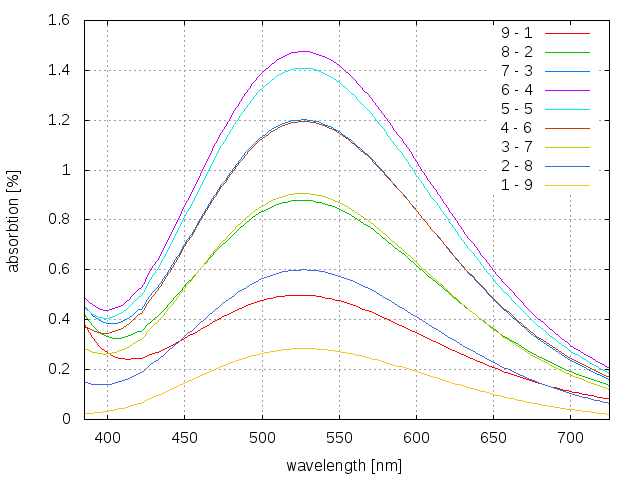
\includegraphics[width=.5\textwidth]{abszorbcios_csucsok.png}
		\caption[Abszorbciós csúcsok]{A vas-amónium szulfát - szalicilsav keverék elnyelési karakterisztikája a keverési arány függvényében. Látható, hogy a hasonló arányú keverékek elnyelési maximuma magasabban van. A legnagyobb abszorpciójú keverék nem az 1Fe-1sal, hanem a 4Fe-6sal arányú volt. \label{fig:absz}}
	\end{figure}\\
	A (\ref{eq:masodfoku}) görbét a \ref{tab:maxes}. táblázatban szereplő pontokra illesztve a következő paramétereket kapjuk:\\
	\begin{tabular}{clll}
		&&&\\
		mennyiség&érték&absz. hiba&rel. hiba\\ [5pt]
		k&24.7212&$\pm 9.672$&(39.13\%)\\
		d&1.46637&$\pm 0.04989$&(3.402\%)\\
		a&3.19525&$\pm 0.1114$&(3.488\%)\\
		&&&\\
	\end{tabular}\\
	\\
	Az anyagmennyiségek arányszáma $d = 1.47$ volt, azaz indokolt volt nem ekvimoláris modellel számolni (ez a mért görbéken is szembetűnő). Az egyensúlyi állandó (\ref{eq:xyz}) alapján (hibája a hozzá tartozó k paraméter hibájából számítható):
	\begin{equation}
	K = \frac{\kappa}{c_0} = \frac{24.72}{2.5\ mM} = (9.86 \pm 3.87) \frac{1}{mM}
	\end{equation}
	\begin{figure}[h!]
		\centering
		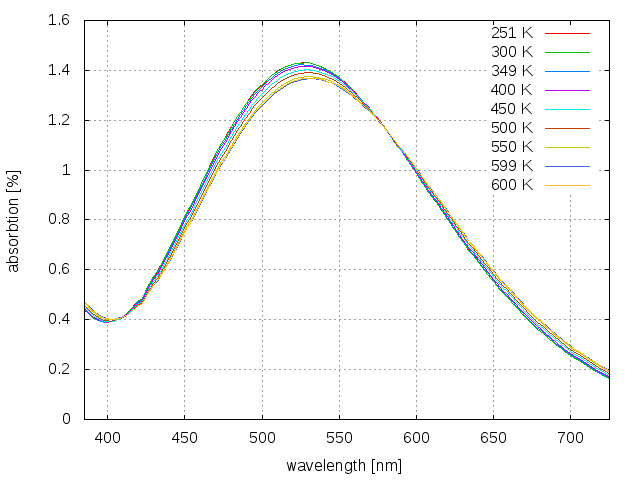
\includegraphics[width=.49\textwidth]{homersekletfugges.png}
		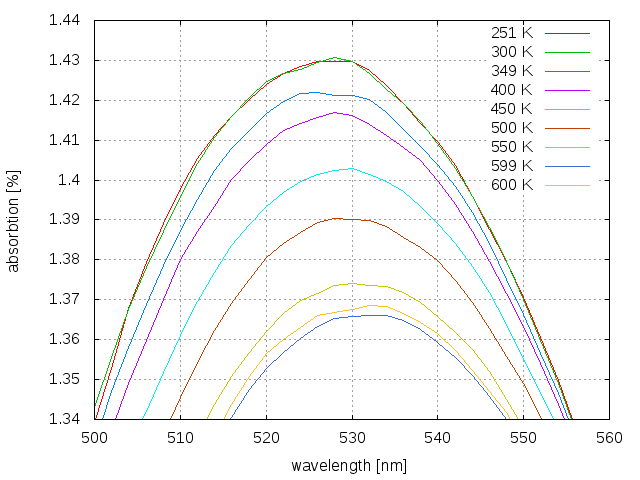
\includegraphics[width=.49\textwidth]{homersekletfuggeszoom.png}
		\caption[Elnyelés hőmérsékletfüggése]{A legnagyobb abszorpciójú, 4Fe-6sal arányú keverék elnyelési spektrumának hőmérsékletfüggése. A jobb oldali ábrán kinagyítva ábrázoltuk a csúcsokat.\label{fig:homfugges}}
	\end{figure}
	\begin{figure}[h!]
		\centering
		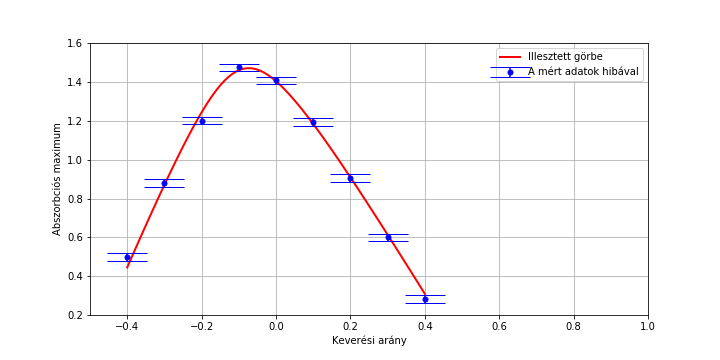
\includegraphics[width=.8\textwidth]{K.png}
		\caption[Másodfokú egyenlet megoldása]{Az abszorcpiós maximum értéke adott keverési arány mellett. Az arányossági paramétereket a görbe illesztésével kaptuk meg. \label{fig:maxes}}
	\end{figure}\\
	\subsection{Extinkciós állandó meghatározása}
	Az így kapott adatok alapján a komplex extinkciós állandója (hibája az a paraméter hibájából számítható):\\
	$$\epsilon=\frac{a}{c_{o}\cdot l}=\frac{3.195}{2.5\ mM\cdot0.01\ m}=(127.8\pm0.11)\ \frac{1}{mM\ m}$$
	\subsection{Egyensúlyi állandó hőmérsékletfüggése}
	A mérést praktikus okokból a legnagyobb abszorbcióval rendelkező, $sal=4, Fe=6$ keverési arányú mintán végeztük. A hőmérsékletet 250K és 600K között 50K-es lépésekben vizsgáltuk. A van't Hoff egyenlet:
	\begin{equation}
	\frac{\partial}{\partial T} ln \frac{K}{c^p_0} = \frac{\Delta h}{k_B T^2}
	\end{equation}
	A differenciálegyenlet megoldása K-ra:
	\begin{equation}
	K (T) = c_1 \cdot e^{-\frac{\Delta h}{c^p_0 k_B} \frac{1}{T}}
	\end{equation}
	(\ref{eq:kappazeta}) alapján $\kappa$ fordítottan arányos a maximumokkal, így azok reciprokát a hőmérséklet függvényében ábrázolva az egyensúlyi állandóra vonatkozó összefüggést kapunk (\ref{fig:tfugges}. ábra). A pontokra egy \texttt{f(x) = x0 + c1 * exp(c2/x)} egyenletű görbét illesztettünk. Az illesztett görbébe egyenletében az exponenciális tag kitevője:
	\begin{equation*}
	c_2 = -1468.88 \pm 226.1 = -\frac{\Delta h}{c^p_0 k_B}
	\end{equation*}
	Ahonnan a reakcióhő (entalpiaváltozás) $\Delta h = (5.09\pm 0.7) \cdot 10 ^{-20} J$ (hibája az illesztési pontatlanság)
	\begin{figure}%[h!]
		\centering
		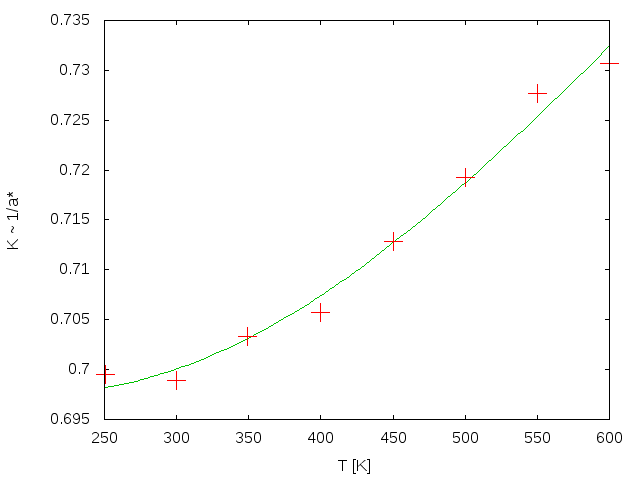
\includegraphics[width=.8\textwidth]{tfugges.png}
		\caption{Az egyensúlyi állandó hőmérsékletfüggése. \label{fig:tfugges}}
	\end{figure}
	
\end{document}